\section{Theoretical Analysis}
\label{sec:analysis}
\paragraph{}
\par In this section, the circuit shown in Figure \ref{circuit} is analysed
theoretically. The known values in $kOhm$, $V$, $mS$, $\mu F$ can be checked in the table below. 
\begin{table}[H]
    \centering
    \begin{tabular}{|c|c|}
    \hline
        $R_1$ & 1.02362892933 \\ \hline 
$R_2$ & 2.08640382129 \\ \hline 
$R_3$ & 3.09996108706 \\ \hline 
$R_4$ & 4.08183334334 \\ \hline 
$R_5$ & 3.04169575790 \\ \hline 
$R_6$ & 2.04156679366 \\ \hline 
$R_7$ & 1.04156790057 \\ \hline 
$C$ & 1.04908336809 \\ \hline 
$K_b$ & 7.29571922963 \\ \hline 
$K_d$ & 8.16840649221 \\ \hline 

    \end{tabular}
    \caption{Known Data}
    \label{data}
\end{table}
\subsection{For $t<0$}
\paragraph{}
\par  For $t<0$, $v_s=V_s$, according to the given equation. Futhermore the capacitor acts like an open circuit since it is fully charged and no current goes through it. Therefore, $I_c = 0$.
\par Applying the node method, it is possible to solve the circuit with the information upwards, since all the other information is given in \ref{circuit}.
The system used to solve this circuit is shown below.
$$
\begin{cases} 
	V_1 = V_s \\ 
	V_d = V_5 -V_8 \\
	V_b = V_2 - V_5 \\
	\frac{V_7 K_d}{R_6} = V_d \\ 
	\frac{V_1 - V_2}{R_1} + \frac{V_3 - V_2}{R_2} - \frac{V_5 - V_2}{R_3}  = 0 \\
	\frac{V_2 - V_3}{R_2} - K_b V_b = 0 \\
	\frac{-V_7}{R_6} + -\frac{V_8 - V_7}{R_7} = 0 \\
	\frac{V_7 - V_8}{R_7} - \frac{V_5}{R_4} + \frac{V_6 - V_5}{R_5} + \frac{V_2 - V_5}{R_3}= 0 \\
	\frac{V_5 - V_6}{R_5} + K_b V_b = 0 
\label{system1}
\end{cases}
$$

Using Octave software it was possible to collect the data shown in table \ref{table1a} and \ref{table1b}.

\begin{table}[H]
    \centering
    \begin{tabular}{|c|c|}
    \hline
        $V_1$ & 5.178860 \\ \hline 
$V_2$ & 4.933049e+00 \\ \hline 
$V_3$ & 4.408850e+00 \\ \hline 
$V_5$ & 4.967487e+00 \\ \hline 
$V_6$ & 5.731699e+00 \\ \hline 
$V_7$ & -1.994280e+00 \\ \hline 
$V_8$ & -3.011723e+00 \\ \hline 
$V_b$ & 3.443737e-02 \\ \hline 
$V_d$ & -7.979210e+00 \\ \hline 
$V_s$ & 5.178860e+00 \\ \hline 

    \end{tabular}
    \caption{Voltages in all nodes in V}
    \label{table1a}
\end{table}

\begin{table}[H]
    \centering
    \begin{tabular}{|c|c|}
    \hline
        $I_1$ & -0.240136 \\ \hline 
$I_2$ & 2.512454e-01 \\ \hline 
$I_3$ & 1.110897e-02 \\ \hline 
$I_4$ & 1.216974e+00 \\ \hline 
$I_5$ & 2.512454e-01 \\ \hline 
$I_6$ & -9.768380e-01 \\ \hline 
$I_7$ & -9.768380e-01 \\ \hline 
$I_b$ & 2.512454e-01 \\ \hline 
$I_d$ & -9.768380e-01 \\ \hline 
$I_s$ & -2.401364e-01 \\ \hline 

    \end{tabular}
    \caption{Currents in all branches in mA}
    \label{table1b}
\end{table}

The voltages and currents were then calculated. 

\subsection{For $t=0$}
\paragraph{}

\par In order to solve the second exercise, firstly it is necessary to replace the capacitor by a voltage source $Vx$, which will impose a voltage of exactly what was determined for the capacitor in the first exercise. This is the first step to compute de $R_eq$ as seen from the capacitor because now it is possible to run a new nodal analysis with $vs$ set to 0 in order to determine $I_x$, which is the current that goes through the capacitor.
\par Solving the matrix below it is possible to determine the values in \ref{system 2} and thus determine $R_{eq}$.

\par Compute $R_{eq}$ is fundamental because this allows to determine the natural solution of the system through the $RC$ constant. This application will be demenstrated in the next exercise.

$$
\begin{cases} 
	V_1 = V_s \\ 
	V_d = V_5 -V_8 \\
	V_b = V_2 - V_5 \\
	V_x = V_6 - V_8 \\
	\frac{V_7 K_d}{R_6} = V_d \\ 
	\frac{V_1 - V_2}{R_1} + \frac{V_3 - V_2}{R_2} - \frac{V_5 - V_2}{R_3}  = 0 \\
	\frac{V_2 - V_3}{R_2} - K_b V_b = 0 \\
	\frac{-V_7}{R_6} -\frac{V_8 - V_7}{R_7} = 0 \\
	\frac{V_7 - V_8}{R_7} - \frac{V_5}{R_4} + \frac{V_6 - V_5}{R_5} + \frac{V_2 - V_5}{R_3} - \frac{V_x}{R_{eq}}= 0 \\
	\frac{V_5 - V_6}{R_5} + K_b V_b + \frac{V_x}{R_{eq}}= 0 
\label{system 2}
\end{cases}
$$



Through Octave it was possible to collect the data shown in table \ref{table2a} and \ref{table2b}.

\begin{table}[H]
    \centering
    \begin{tabular}{|c|c|}
    \hline
        $V_1$ & 0.000000 \\ \hline 
$V_2$ & -6.049490e-16 \\ \hline 
$V_3$ & -1.440730e-15 \\ \hline 
$V_5$ & -1.195182e-15 \\ \hline 
$V_6$ & 8.743422e+00 \\ \hline 
$V_7$ & 1.804316e-15 \\ \hline 
$V_8$ & 2.724843e-15 \\ \hline 
$V_b$ & 5.490679e-17 \\ \hline 
$V_d$ & 3.920025e-15 \\ \hline 
$V_s$ & 0.000000e+00 \\ \hline 
$V_x$ & 8.743422e+00 \\ \hline 

    \end{tabular}
    \caption{Voltages in all nodes in V}
    \label{table2a}
\end{table}


\begin{table}[H]
    \centering
    \begin{tabular}{|c|c|}
    \hline
        $I_1$ & -0.000000 \\ \hline 
$I_2$ & 7.525891e-18 \\ \hline 
$I_3$ & -1.904001e-16 \\ \hline 
$I_4$ & -2.928052e-16 \\ \hline 
$I_5$ & 2.874522e+00 \\ \hline 
$I_6$ & 4.799008e-16 \\ \hline 
$I_7$ & 4.799008e-16 \\ \hline 
$I_b$ & 4.005845e-16 \\ \hline 
$I_d$ & 4.799008e-16 \\ \hline 
$I_s$ & -5.909846e-16 \\ \hline 
$I_x$ & 2.874522e+00 \\ \hline 

    \end{tabular}
    \caption{Currents in all branches in mA}
    \label{table2b}
\end{table}




\par The value for $V_x$ was estabilished as $V_6 - V_8$ being $V_6$ and $V_8$ determined in the previous section.

\subsection{Natural Solution}
\paragraph{}

\par Now the task was to determine the natural solution for $V_6$. Using $V_x$, determined in the previous exercise, as the initial condition, it was possible, applying \ref{equationnat}, since this is a RC circuit, to determine the natural solution, plotted in figure \ref{natural ana}.

\begin{equation}
	V_{6n} = A e^{\frac{-t}{\tau}}  \ \ \  \ \ \ \ \tau = R_{eq} C
	\label{equationnat}
\end{equation}



\begin{figure}[H]
    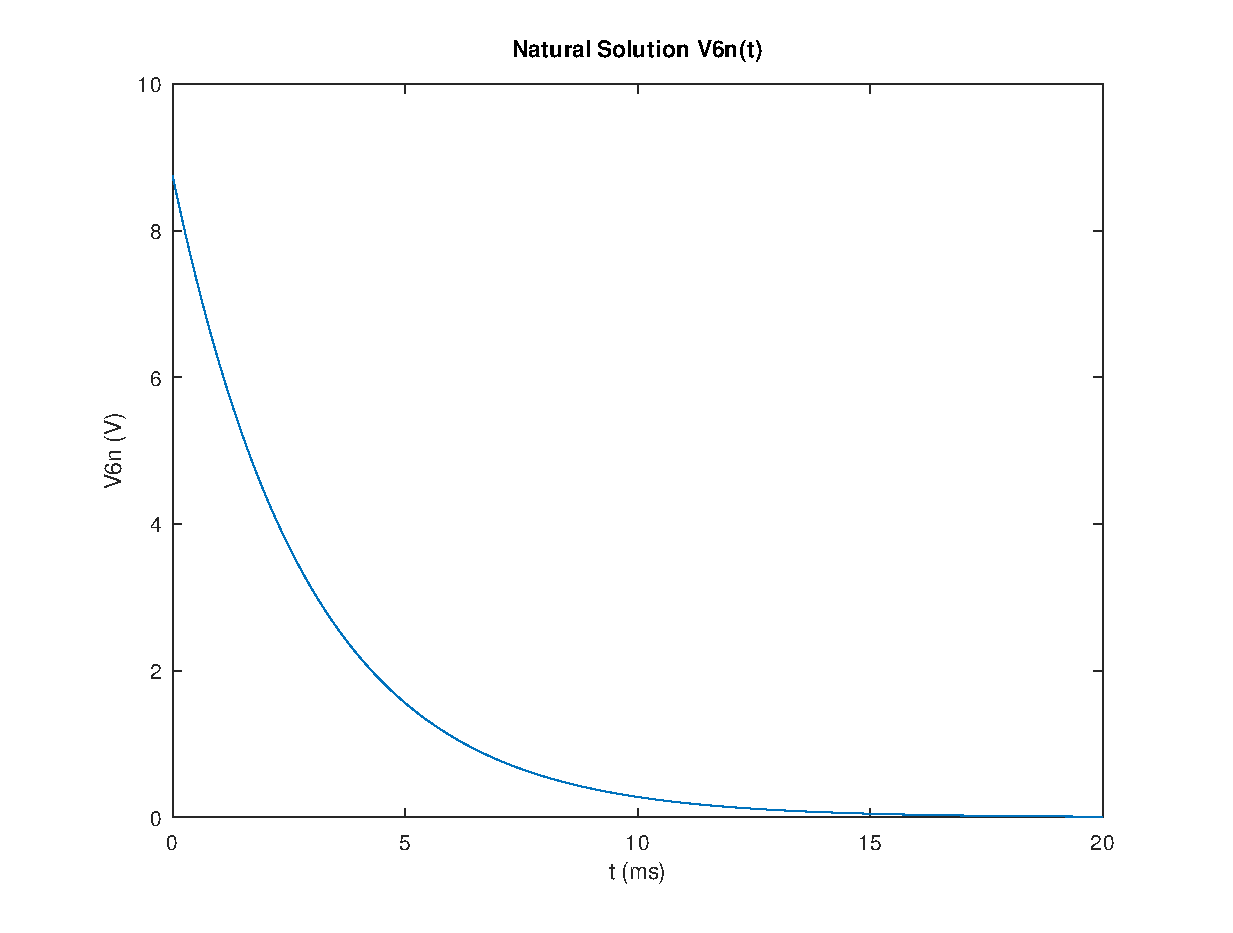
\includegraphics[width=0.5\linewidth]{naturalana.eps}
    \centering
    \caption{Natural Solution}
    \label{natural ana}
\end{figure}

\subsection{Forced Solution}
\paragraph{}

\par For this section of the analysis, one was asked to find the forced solution $V_{6}f(t)$ for a frequency of 1000Hz. In order to simplify the calculations, and as suggested, a phasor with constant $V_s$ of 1V was used.
A similar node analysis was ran, using $V_s$ as the voltage source, and replacing the capacitance of capacitor $C$ with its impendance $Z$. Like so, the following nodal equations were derived:

\begin{equation}
	Z_c = \frac{1}{j \omega C}     \ \ \  \ \ \ \ \  \ \ \ \ \ \ \ \omega = 2 \pi f
\end{equation}


$$
\begin{cases} 
	V_1 = V_s \\ 
	V_d = V_5 -V_8 \\
	V_b = V_2 - V_5 \\
	\frac{V_7 K_d}{R_6} = V_d \\ 
	\frac{V_1 - V_2}{R_1} + \frac{V_3 - V_2}{R_2} - \frac{V_5 - V_2}{R_3}  = 0 \\
	\frac{V_2 - V_3}{R_2} - K_b V_b = 0 \\
	\frac{-V_7}{R_6} -\frac{V_8 - V_7}{R_7} = 0 \\
	\frac{V_7 - V_8}{R_7} - \frac{V_5}{R_4} + \frac{V_6 - V_5}{R_5} + \frac{V_2 - V_5}{R_3} - \frac{V_6 - V_8}{Z_c}= 0 \\
	\frac{V_5 - V_6}{R_5} + K_b V_b + \frac{V_8 - V_6}{Z_c}= 0 
\label{system 4}
\end{cases}
$$
\par Spliting the complex numbers and determining the angles and the modules, the two following rables were made with the following equations:

\begin{equation}
	V_{complex_i} = V_i e^{-j phase(i)}
\end{equation}

\par With angle and abs commands in octave we were able to calculate the following values.

\begin{table}[H]
    \centering
    \begin{tabular}{|c|c|}
    \hline
        $V_1$ & 1.000000e+00 \\ \hline 
$V_2$ & 9.531327e-01 \\ \hline 
$V_3$ & 8.616507e-01 \\ \hline 
$V_5$ & 9.471228e-01 \\ \hline 
$V_6$ & 5.742283e-01 \\ \hline 
$V_7$ & 3.802382e-01 \\ \hline 
$V_8$ & 5.742283e-01 \\ \hline 

    \end{tabular}
    \caption{Complex Amplitudes}
    \label{table4a}
\end{table}

\paragraph{}

\begin{table}[H]
    \centering
    \begin{tabular}{|c|c|}
    \hline
        $Ph_1$ & 0.000000e+00 \\ \hline 
$Ph_2$ & -3.749681e-21 \\ \hline 
$Ph_3$ & -1.224400e-20 \\ \hline 
$Ph_5$ & -4.257358e-21 \\ \hline 
$Ph_6$ & 3.141434e+00 \\ \hline 
$Ph_7$ & 3.141593e+00 \\ \hline 
$Ph_8$ & 3.141593e+00 \\ \hline 

    \end{tabular}
    \caption{Phases}
    \label{table4b}
\end{table}


Therefore, we can state that:

\begin{equation}
	V_6 = 5.742283e-01 e^{-j 3.141434e+00}
\end{equation}

\subsection{Natural and Forced Superimposed}
\paragraph{}

\par By converting the phasor to real time functions, a function to evaluate $V_6$, for $t>0$, was found by simply adding the natural and forced solutions, previously calculated for a frequency of 1000Hz. On the other hand, the equation for $V_s(t)$ for $t>0$ was already implicit on the initial circuit diagram. Both equations are written below.

\begin{equation}
	V_{ifinal} = V_{in} + V_{if}
\end{equation}

So, calculating $V_{6final}$:
\begin{equation}
	V_{6}(t) = e^{\frac{-t}{R_{eq} C}} + A e^{-j phase(i)}
\end{equation}

\begin{figure}[H]
    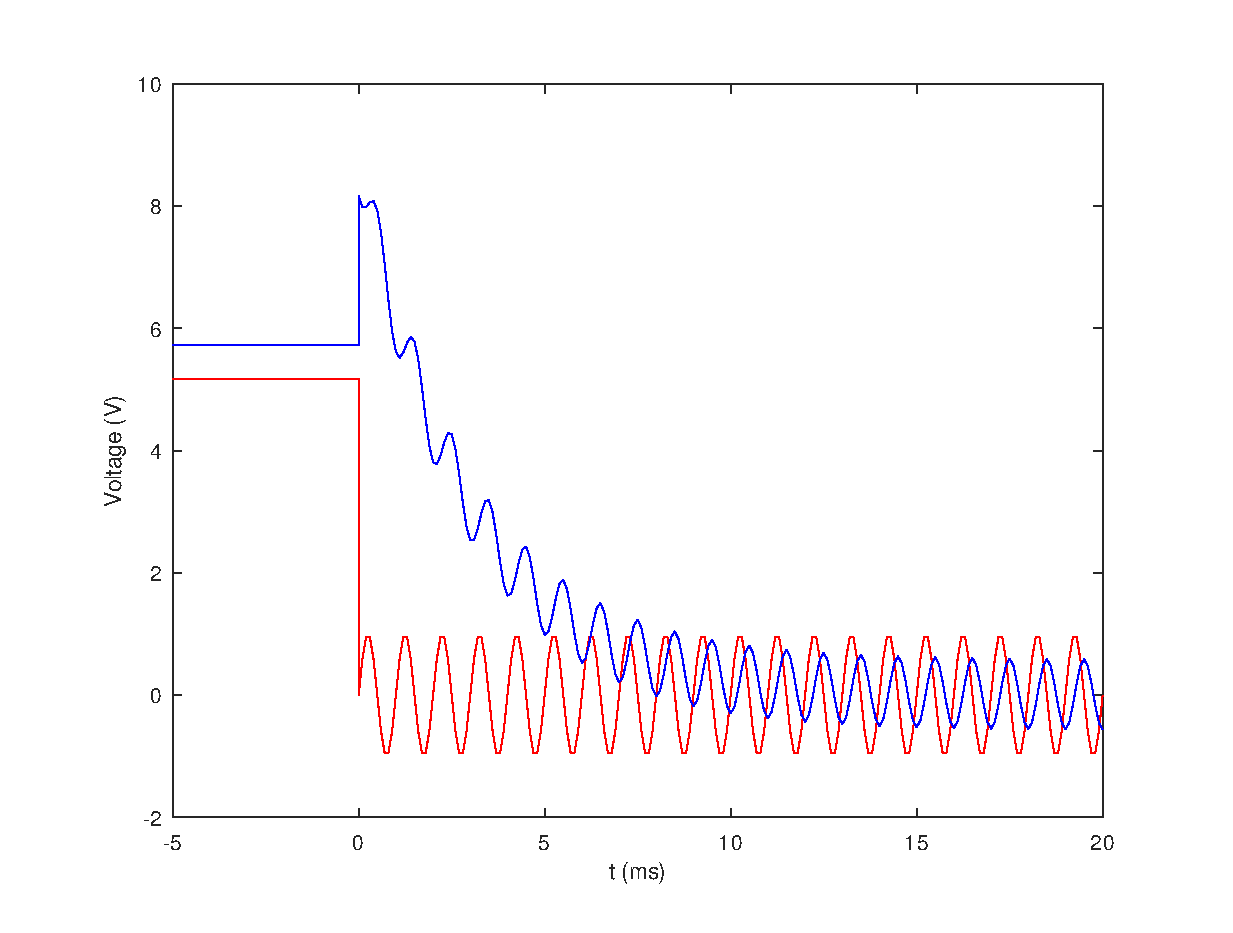
\includegraphics[width=0.5\linewidth]{5ex.eps}
    \centering
    \caption{Natural and Forced Superimposed}
    \label{pha}
\end{figure}




\subsection{Frequency Response}
\paragraph{}

\par The graphs for phase and magnitude were plotted. The magnitude in dB is calculated with the help of the function abs and in a logarthmic scale, multiplied by the 20. The phase in degrees is calculated with the function angle and there has to be a conversion from rad to degrees.
\begin{equation}
	Z=\frac{1}{j 2 \pi f C}
\end{equation}

with $f$ being a logharitmic scale vector from -6 to 6 with 200 entries.

The system used was:

$$
\begin{cases} 
	V_1 = V_s \\ 
	V_d = V_5 -V_8 \\
	V_b = V_2 - V_5 \\
	\frac{V_7 K_d}{R_6} = V_d \\ 
	\frac{V_1 - V_2}{R_1} + \frac{V_3 - V_2}{R_2} - \frac{V_5 - V_2}{R_3}  = 0 \\
	\frac{V_2 - V_3}{R_2} - K_b V_b = 0 \\
	\frac{-V_7}{R_6} -\frac{V_8 - V_7}{R_7} = 0 \\
	\frac{V_7 - V_8}{R_7} - \frac{V_5}{R_4} + \frac{V_6 - V_5}{R_5} + \frac{V_2 - V_5}{R_3} - \frac{V_6 - V_8}{Z}= 0 \\
	\frac{V_5 - V_6}{R_5} + K_b V_b + \frac{V_8 - V_6}{Z}= 0 
\label{system 6}
\end{cases}
$$

The complex variables $Vsfre(k)$, $Vxfre(k)$ and $V6fre(k)$ were assigned and equalled to the just calculated $V_1$, $V_6 - V_8$ and $V_6$, respectively. 

The two following graphics were plotted using a base 10 logarithmic scale for frequencies, the logarithmic value of the $abs$ of the variables stated above and the angle of these complex variables, converted to degrees.



\begin{figure}[H]
    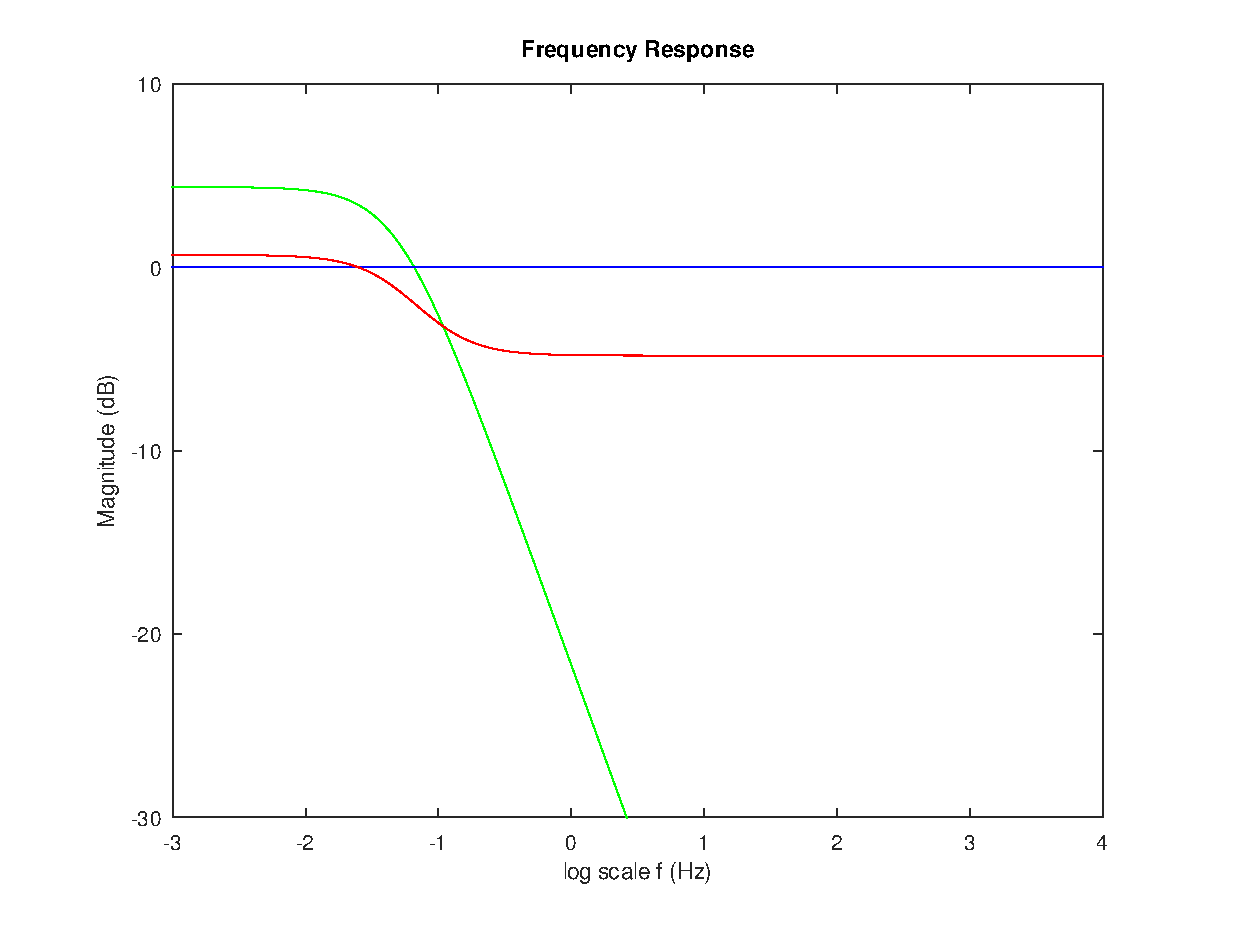
\includegraphics[width=0.5\linewidth]{ex6mag.eps}
    \centering
    \caption{Magnitude (dB) / Frequency (Hz)}
    \label{mag}
\end{figure}

\begin{figure}[H]
    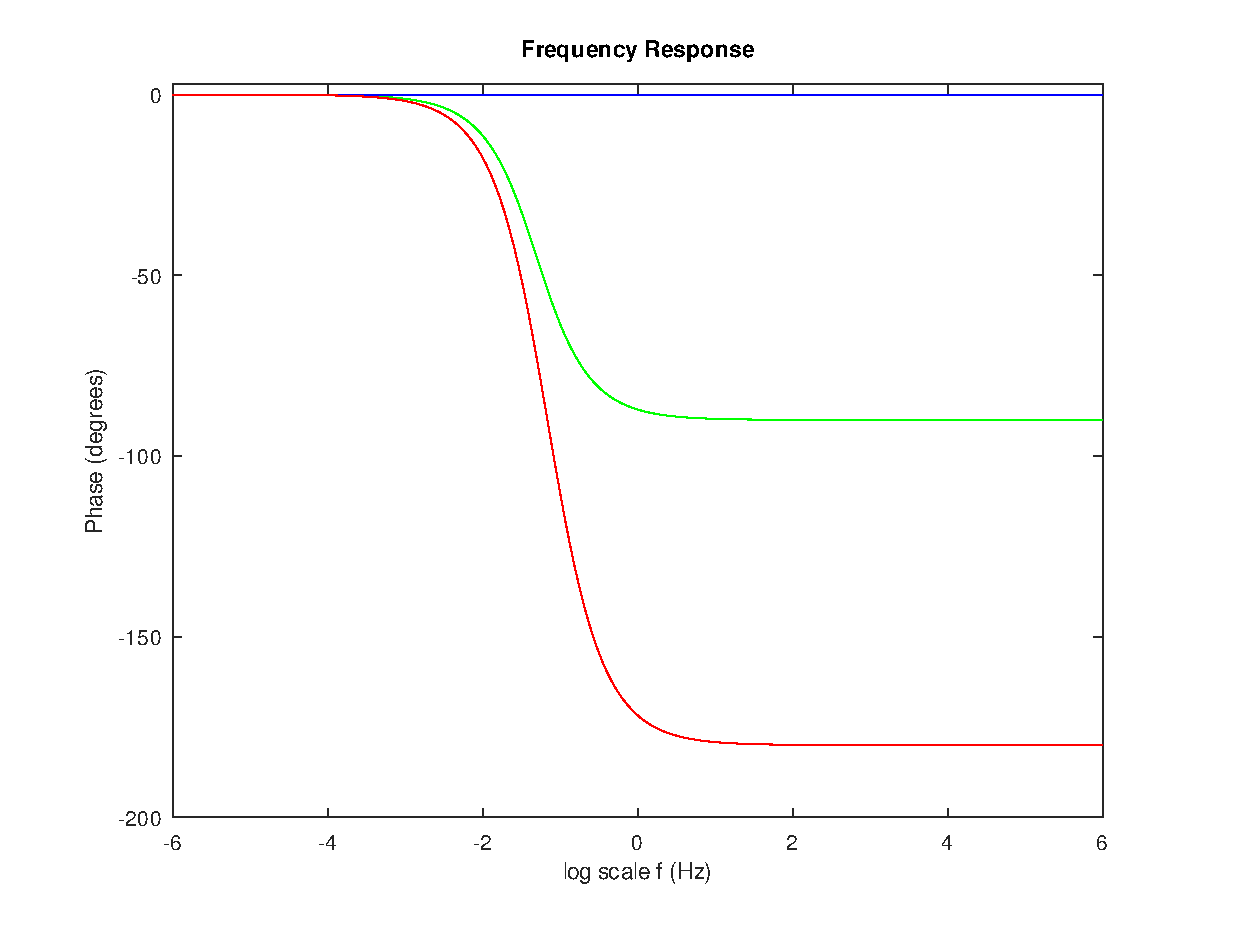
\includegraphics[width=0.5\linewidth]{ex6pha.eps}
    \centering
    \caption{Phase (degrees) / Frequency (Hz)}
    \label{pha}
\end{figure}


